\addtocontents{toc}{\vspace{2em}}
\chapter{Υλοποίηση του συστήματος} % Main chapter title

\label{Chapter7} 

\section{Γενικά}
 Σε αυτή την ενότητα θα γίνει μία εκτενής περιγραφή στην ανάπτυξη του συστήματος ελέγχου του σιλό σύμφωνα με τις προδιαγραφές που αναφέρθηκαν παραπάνω. Η υλοποίηση του συστήματος ελέγχου έγινε σε Java χρησιμοποιώντας την component-based προσέγγιση για την ανάπτυξη του λογισμικού. Χρησιμοποιήθηκε το OSGi framework καθώς παρείχε αρκετά πλεονεκτήματα και αρκετές υπηρεσίες που κρίθηκαν πολύ βοηθητικές. Επιπλέον, χρησιμοποιώντας Java για την ανάπτυξη του συστήματος ελέγχου έχουμε αρκετές επιλογές για το υλικό που μπορεί να χρησιμοποιηθεί καθώς η συγκεκριμένη γλώσσα μπορεί να τρέξει σε μεγάλο εύρος συσκευών. Επιπλέον, επιλέγοντας την συγκεκριμένη γλώσσα προγραμματισμού δίνεται η δυνατότητα χρήσης δύο βιβλιοθηκών που υλοποιούν τα πρωτόκολλα CoAP και LwM2M, τις Californium και Leshan αντίστοιχα, καθώς και της βιβλιοθήκης pi4j [60] που μας επιτρέπει να χρησιμοποιήσουμε τα γενικού σκοπού I/O του Raspberry Pi μέσω της Java. 

	Στην συγκεκριμένη εργασία χρησιμοποιήθηκαν σαν ενσωματωμένοι μικροϋπολογιστές  Raspberry Pi 3 Model B και Raspberry Pi 2 Model B.  Η υλοποίηση του συστήματος ελέγχου έγινε στο Intellij IDEA IDE της Jetbrains καθώς υπήρχε άδεια για την χρησιμοποίηση της έκδοσης  Ultimate μέσω του Πανεπιστημίου. Tέλος χρησιμοποιήθηκε το σύστημα ελέγχου πηγαίου κώδικα Git σε συνδυασμό με την υπηρεσία Github. 
	
\section{Οι συνιστώσες του συστήματος ελέγχου}
Όπως έχει ήδη αναφερθεί, η υλοποίηση του λογισμικού του συστήματος έγινε χρησιμοποιώντας την προσέγγιση συνιστωσών με την βοήθεια του OSGi framework. Για να γίνει κάτι τέτοιο έπρεπε αρχικά να ξεχωριστούν οι διάφορες συνιστώσες του συστήματος. Φυσικά και το σύστημα ελέγχου θα μπορούσε να υλοποιηθεί σε ένα μόνο component. Κάτι τέτοιο όμως θα σήμαινε ότι το σύστημα ελέγχου θα υλοποιούνταν σαν ένα Plain Old Java Object (POJO) και ως συνέπεια δεν θα μπορούσαμε να επωφεληθούμε από τα πλεονεκτήματα που μας προσφέρει το OSGi. Κατά συνέπεια αποφασίστηκε το σύστημα ελέγχου να αποτελείται από πολλές συνιστώσες, όπου κάθε μία θα είναι υπεύθυνη για μία λειτουργία του σιλό. Στην εικόνα 7.1 φαίνονται οι συνιστώσες από τις οποίες αποτελείται το σύστημα. Το διάγραμμα αυτό είναι ένα component διάγραμμα όπως το προτείνει η OSGi Alliance [48] και δείχνει τη δομή του cyber μερους του σιλό ως Industrial Automation Thing. Κάθε συνιστώσα σε αυτό το διάγραμμα αντιστοιχεί σε ένα φυσικό μέρος του σιλό το οποίο μπορεί να αντικατασταθεί ανά πάσα στιγμή. 

	Ένα πολύ σημαντικό χαρακτηριστικό του OSGi είναι ότι οι διάφορες συνιστώσες του συστήματος θα πρέπει να επικοινωνούν μεταξύ τους μέσω καλά καθορισμένων interfaces. Έτσι κάθε συνιστώσα πρέπει να εξάγει τις διεπαφές που είναι απαραίτητες ώστε να επικοινωνήσει με το περιβάλλον της και κάποια άλλη συνιστώσα να μπορεί να επικοινωνήσει με αυτή. Στο διάγραμμα μπορούμε να παρατηρήσουμε ότι κάθε .api συνιστώσα εξάγει το πακέτο που περιέχει τα διάφορα interfaces της. Το πακέτο που εξάγεται εμφανίζεται στο διάγραμμα σαν ένα μαύρο κουτί μέσα στο component, ενώ τα πακέτα που το  κάθε component απαιτεί ώστε να μπορέσει να λειτουργήσει μοντελοποιούνται σαν λευκά κουτιά. Για παράδειγμα, η συνιστώσα valve.out υλοποιεί την λειτουργικότητα του driver της βαλβίδας εξαγωγής υγρού του σιλό και η συνιστώσα valve.out.api καθορίζει τις υπηρεσίες που παρέχει η βαλβίδα εξαγωγής υγρού στον περιβάλλον της. Ο controller του σιλό στην εικόνα 7.1 πρέπει να χρησιμοποιήσει τις .api συνιστώσες των τριών drivers, δηλαδή του siloDriver που είναι υπεύθυνος για την λειτουργικότητα των αισθητήρων,  του inValveDriver  και του outValveDriver που είναι υπεύθυνοι για την λειτουργικότητα της βαλβίδας εισαγωγής και εξαγωγής υγρού αντίστοιχα. Στη συνέχεια θα γίνει μία εκτενέστερη ανάλυση του τρόπου λειτουργίας της κάθε συνιστώσας καθώς και του τρόπου χρήσης του OSGi.
	
\begin{figure}[htbp]
	\centering
		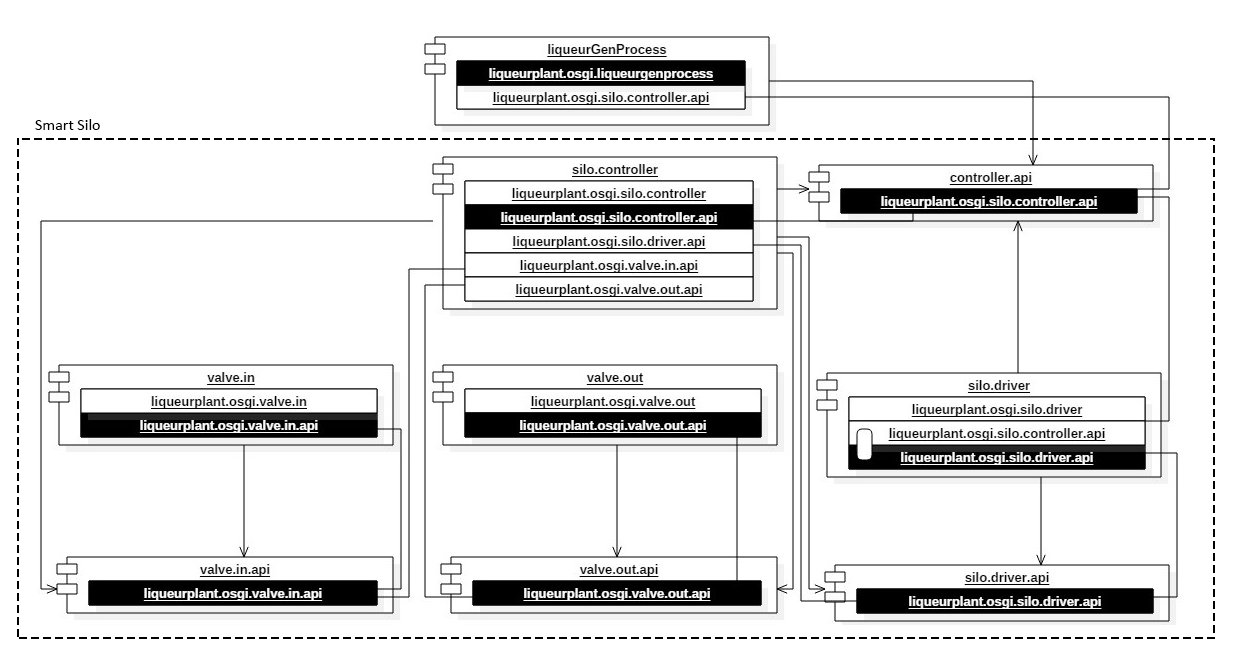
\includegraphics[height=10cm,width=16cm]{Figures/21.png}
	\caption{Το διάγραμμα συνιστωσών ενός σιλό}	
\end{figure}

\section{Ανάλυση των συνιστωσών του συστήματος ελέγχου}

\subsection{Οι συνιστώσες των drivers του σιλό}
Όπως περιγράφηκε και στην προηγούμενη ενότητα, κάθε συνιστώσα είναι υπεύθυνη για την λειτουργικότητα ενός φυσικού στοιχείου του σιλό. Αυτό σημαίνει ότι για κάθε στοιχείο που εκτελεί ένα έργο για το σύστημα θα υπάρχει ένα component υπεύθυνο για την υλοποίηση και ένα component υπεύθυνο για τις υπηρεσίες που εξάγει στο περιβάλλον του. Έτσι έχουμε την ακόλουθη αντιστοίχηση φυσικών μερών του συστήματος με συνιστώσες λογισμικού που φαίνεται στον πίνακα 7.1:


\begin{table}[h]
\centering
\begin{tabular}{|c|c|}
\hline
\textbf{Φυσικό Μέρος του Σιλό} & \textbf{Component λογισμικού} \\ \hline
Βαλβίδα εισαγωγής υγρού & Valve.in \\ \hline
Βαλβίδα εξαγωγής υγρού & Valve.out \\ \hline
Στοιχείο ανάδευσης του υγρού & Mixer.driver \\ \hline
Στοιχείο θέρμανσης του υγρού & Heater.driver \\ \hline
Αισθητήρες επιπέδου υγρού & Silo.driver \\ \hline
\end{tabular}
\caption{Αντιστοίχηση των φυσικών μερών του σιλό με τη συνιστώσα τους}
\label{my-label}
\end{table}

\subsubsection{Συνιστώσες βαλβίδων του σιλό}
	Είναι υπεύθυνες για την αντιστοίχηση του μηχανικού μέρους της βαλβίδας του σιλό σε επίπεδου λογισμικού ώστε να μπορεί να χρησιμοποιηθεί από τον ενσωματωμένο μικροϋπολογιστή και να παρέχει τις υπηρεσίες που περιγράφηκαν στο κεφάλαιο 6 στο περιβάλλον του. Γι’ αυτό οι συγκεκριμένες συνιστώσες αποτελούνται από μία διεπαφή (.api component) μέσω τις οποίας παρέχουν στον περιβάλλον τους υπηρεσίες για το άνοιγμα και το κλείσιμο της βαλβίδας. Αυτές οι διεπαφές υλοποιούνται από τα components valve.in και valve.out όπου με την βοήθεια της βιβλιοθήκης pi4j αποστέλνεται σήμα στην βαλβίδα να ανοίξει ή να κλείσει ανάλογα με την περίπτωση.  Η διεπαφή των βαλβίδων αποτελείται από το interface ValveDriverIf το οποίο ορίζει τις μεθόδους open() και close() οι οποίες ανοίγουν και κλείνουν την βαλβίδα αντίστοιχα. Στο component που υλοποιεί αυτή τη λειτουργικότητα έχουμε την υλοποίηση αυτών των μεθόδων, όπου κάθε μέθοδος αλλάζει την τάση σε ένα συγκεκριμένο γενικού σκοπού I/O του Raspberry Pi. Αξίζει επίσης να σημειωθεί ότι χρησιμοποιήθηκαν και όροι OSGi ώστε να μπορεί αυτή η υλοποίηση να είναι component. Αυτό γίνεται χρησιμοποιώντας το annotation \textbf{@Component} μέσα στο οποίο ορίζεται το όνομα της συνιστώσας καθώς και το όνομα της υπηρεσίας που απαιτεί για να λειτουργήσει. Αυτά φαίνονται καλύτερα και στον αλγόριθμο 7.1 όπου βλέπουμε την υλοποίηση του component για την βαλβίδα εξαγωγής υγρού από το σιλό. 

\newpage

\begin{lstlisting}[caption=Μέρος της υλοποίησης της συνιστώσας την βαλβίδας εξαγωγής υγρού]
$$@Component(
        name = "liqueurplant.osgi.valve.out",
        service = liqueurplant.osgi.valve.out.api.OutValveDriverIf.class
)
public class OutValveDriver implements OutValveDriverIf {
	.
	.
	.
    $$@Override
    public void open() throws Exception {
        try {
            outValvePin.setState(PinState.LOW);
        } catch (Exception e) {
            LOGGER.error("Exception in open(): " + e.toString());
        }
    }

    $$@Override
    public void close() throws Exception {
        try {
            outValvePin.setState(PinState.HIGH);
        } catch (Exception e) {
            LOGGER.error("Exception in close(): " + e.toString());
        }
    }
}
\end{lstlisting}

\subsubsection{Συνιστώσες στοιχείων θέρμανσης και μίξης του σιλό}
Είναι υπεύθυνες για την λειτουργικότητα των στοιχείων ανάδευσης και θέρμανσης του υγρού που μπορεί να περιέχει κάποιο σιλό. Σχετικά με το στοιχείο ανάδευσης του υγρού, αποτελείται από ένα .api component μέσω του οποίου παρέχει τις υπηρεσίες έναρξης και τερματισμού λειτουργίας του μηχανικού μέρους για την ανάδευση του υγρού. Αυτές οι υπηρεσίες παρέχονται μέσω ενός interface στον περιβάλλον του σιλό, το MixerDriverIf και υλοποιούνται από το mixer component στο οποίο όταν έρθει εντολή για έναρξη ανάδευσης το υγρό αναμειγνύεται για συγκεκριμένο χρόνο και η διαδικασία αυτή σταματάει όταν έρθει εντολή τερματισμού. Πάλι και εδώ χρησιμοποιούνται τα αντίστοιχα annotations ώστε το περιβάλλον του OSGi να μπορεί να αναγνωρίζει τη συγκεκριμένη συνιστώσα σαν component. Για το στοιχείο θέρμανσης ακολουθήθηκε παρόμοια λογική, πέρα από το γεγονός ότι υλοποιήθηκε και ένα callback καθώς ήταν απαραίτητη η εισαγωγή πληροφορίας από το μηχανικό μέρος του σιλό. Έτσι μόλις ο αισθητήρας θερμοκρασίας του σιλό επιστρέψει την επιθυμητή τιμή καλείται η μέθοδος heatingCompleted ώστε να σταματήσει η διαδικασία θέρμανσης του υγρού. Στον αλγόριθμο 7.2 φαίνονται οι υπηρεσίες που παρέχει η συνιστώσα του στοιχείου θέρμασης του σιλό στον περιβάλλον της. 


\begin{lstlisting}[caption=Οι υπηρεσίες που παρέχει η συνιστώσα του στοιχείου θέρμανσης]
$$@ProviderType
public interface HeaterDriverIf {
    void start();
    void stop();
    void heat2temp(float temperature);
    void addHeatingCompletedListener(HeatingCompletedListenerIf listener);
}

\end{lstlisting}

Με τη χρήση του annotation \textbf{@ProviderType} οι υπηρεσίες αυτές εγγράφονται στο μητρώο υπηρεσίων του OSGi και μπορούν να χρησιμοποιηθούν από άλλες συνιστώσες.


\subsubsection{Συνιστώσα του driver του σιλό}
Ο συγκεκριμένος driver είναι υπεύθυνος για τους αισθητήρες επιπέδου του υγρού. Η συγκεκριιμένη συνιστώσα δεν συνοδεύεται από ένα component .api καθώς δεν μπορεί να εξάγει κάποια υπηρεσία. Αυτό έγινε γιατί αντιμετωπίστηκε το πρόβλημα των κυκλικών εξαρτήσεων μεταξύ του συστήματος ελέγχου και της συνιστώσας του driver του σιλό. Γι’ αυτό το λόγο ακολουθήθηκε μία διαφορετική προσέγγιση κατά την οποία ο driver επικοινωνεί με τον controller μέσω της EventQueue του controller. Για να γίνει αυτό πιο σαφές, ας θεωρήσουμε ότι το σιλό βρίσκεται στην κατάσταση FILLING. Όταν το υγρό φτάσει στο ανώτατο σημείο του σιλό τότε ο άνω αισθητήρας ανίχνευσης υγρού θα ενεργοποιηθεί και ο driver θα εισάγει στην EventQueue του controller ένα μήνυμα ότι το σιλό έχει γεμίσει ώστε το σύστημα ελέγχου να συνεχίσει τις απαραίτητες διαδικασίες ώστε να λειτουργήσει σωστά όλο το σύστημα παραγωγής. Κάτι τέτοιο δημιουργεί την ανάγκη η συνιστώσα του driver να χρειάζεται τις υπηρεσίες που παρέχει η συνιστώσα του controller για να λειτουργήσει. Αυτό φαίνεται και από το reference που υπάρχει στην συνιστώσα του controller στην υλοποίηση του driver που φαίνεται στον αλγόριθμο 7.3. 
\begin{lstlisting}[caption=Μέρος της υλοποίησης της συνιστώσας του driver του σιλό]

$$@Component(
        name = "liqueurplant.osgi.silo.driver",
        immediate = true
)
public class SimpleSiloDriver {
   .
   .
   .
    $$@Reference(
            policy = ReferencePolicy.DYNAMIC,
            cardinality = ReferenceCardinality.OPTIONAL
    )
    protected void setSiloCtrlIf(SiloCtrlIf siloCtrl) {
        this.siloCtrl = siloCtrl;
        LOGGER.info("SILO-CONTROLLER binded.");
    }

    protected void unsetSiloCtrlIf(SiloCtrlIf siloCtrl) {
        this.siloCtrl = null;
        LOGGER.info("SILO-CONTROLLER unbinded.");
    }
}
\end{lstlisting}

Από μερίας λογισμικού, ο driver του σιλό υλοποιεί δύο \textbf{Listeners} με την βοήθεια της βιβλιοθήκης Pi4j, και συγκεκριμένα του interface GpioPinListenerDigital. Ο listener που αφορά την ακίδα που είναι υπεύθυνη για τον άνω αισθητήρα παρουσίας υγρού του σιλό περιμένει να λάβει σήμα υψηλής τάσης στο γενικού σκοπού I/O του Raspberry Pi από τον εξομοιωτή του σιλό. Όταν έρθει το συγκεκριμένο σήμα τότε εισάγει στην EventQueue του σιλό ένα νέο Signal ότι το υγρό έχει γεμίσει το σιλό. Ομοίως υπάρχει και ένας Listener για  τον κάτω αισθητήρα παρουσίας υγρού του σιλό. Η υλοποίηση αυτή φαίνεται και στον αλγόριθμο 7.4. Αξίζει να σημειωθεί ότι το annotation \textbf{@Activate} που υπάρχει στο πάνω μέρος της μεθόδου, αποτελεί μέρος του OSGi framework και αφορά τον κύκλο ζωής της συγκεκριμένης συνιστώσας. Έτσι μόλις ενεργοποιηθεί η συγκεκριμένη συνιστώσα θα τρέξει η μέθοδος αυτή ώστε να γίνουν οι απαραίτητες αρχικοποιήσεις.
\newpage
\begin{lstlisting}[caption=Η υλοποίση των listener του driver του σιλό]
$$@Activate
public void activate() {
	highLevelSensorPin = gpioController.provisionDigitalInputPin(RaspiPin.GPIO_02, "HIGH-LEVEL-SENSOR", PinPullResistance.PULL_DOWN);
	lowLevelSensorPin = gpioController.provisionDigitalInputPin(RaspiPin.GPIO_03, "LOW-LEVEL-SENSOR", PinPullResistance.PULL_DOWN);

	highLevelSensorPin.setShutdownOptions(true);
	lowLevelSensorPin.setShutdownOptions(true);

	highLevelSensorPin.addListener((GpioPinListenerDigital) event -> {
		if (event.getState() == PinState.HIGH) {
			siloCtrl.put2MsgQueue(new HighLevelReachedSignal());
		}
	});
	lowLevelSensorPin.addListener((GpioPinListenerDigital) event -> {
		if (event.getState() == PinState.LOW) {
			siloCtrl.put2MsgQueue(new LowLevelReachedSignal());
		}
	});
}
\end{lstlisting}

\subsubsection{Συνιστώσα του controller του σιλό}
Αποτελεί το βασικό μέρος του συστήματος ελέγχου, καθώς όλα τα μηνύματα που έρχονται τόσο από τον LwM2M server όσο και από τους drivers του σιλό πρέπει να επεξεργαστούν από τον συγκεκριμένο μέρος του συστήματος. Η συγκεκριμένη συνιστώσα του συστήματος περιλαμβάνει μία EventQueue μέσα στην οποία μπορούν να τοποθετηθούν διάφορα μηνύματα που αφορούν τη λειτουργία του σιλό. Ένα άλλο σημαντικό κομμάτι της υλοποίησης είναι το Generic State Machine που χρησιμοποιήθηκε στον controller του σιλό. 

Αυτό το state machine έχει υλοποιηθεί σε άλλη διπλωματική εργασία που έγινε παράλληλα με την εκπόνηση της παρούσας και χρησιμοποιείται στο controller του σιλό ώστε να γίνεται η επεξεργασία των μηνυμάτων που λαμβάνει καθώς και οι κατάλληλες ενέργειες που απαιτούνται ώστε να επιτευχθεί σωστή λειτουργία του συστήματος ελέγχου. Έχει υλοποιηθεί με μοντέλο την μηχανή καταστάσεων της UML. Αυτό σημαίνει ότι πρέπει να δηλωθούν οι διαφορετικές καταστάσεις στις οποίες μπορεί να βρεθεί το σιλό καθώς και οι διάφορες μεταβάσεις από την μία κατάσταση στην άλλη. Κάθε κατάσταση περιέχει τρεις μεθόδους τις entry, doActivity, exit όπως ακριβώς ορίζει και η UML. Σε αυτές τις μεθόδους εκτελούνται ενέργειες όταν το σιλό εισέλθει σε μία νέα κατάσταση, κατά την διάρκεια που βρίσκεται σε αυτή και πριν μεταβεί σε κάποια επόμενη κατάσταση αντίστοιχα. Σε αυτές τις μεθόδους βρίσκεται το μεγαλύτερο μέρος της λογικής του συστήματος ελέγχου. 

	
	Ο controller του συστήματος παρέχει μέσω της .api συνιστώσας υπηρεσίες υπεύθυνες για την εισαγωγή και εξαγωγή μηνυμάτων από την EventQueue του, οι οποίες φαίνονται στον αλγόριθμο 7.5. Αξίζει να σημειωθεί ότι η EventQueue υλοποιήθηκε με την χρήση της τεχνολογίας ArrayBlockingQueue που μας παρείχε η Java καθώς θα έπρεπε να χρησιμοποιείται από δύο νήματα που θα τρέχουν ταυτόχρονα. Κάτι τέτοιο μας έδωσε την δυνατότητα να μην πέσουμε σε κάποιο deadlock και τα νήματα τόσο του controller όσο και του LwM2M client να λειτουργούν χωρίς να παρουσιαστεί κάποιο πρόβλημα. 

	Η συγκεκριμένη συνιστώσα πρέπει ανάλογα με τον τύπο του σιλό να περιμένει να λάβει τις υπηρεσίες από τα διάφορα άλλα components όπως για παράδειγμα των βαλβίδων και του driver του σιλό. 
	
\begin{lstlisting}[caption=Οι υπηρεσίες που παρέχει η συνιστώσα του ελεγκτή του σιλό]
$$@ProviderType
public interface SiloCtrlIf {
    void put2MsgQueue(BaseSignal signal);
    BaseSignal takeNotification();
}

\end{lstlisting}


\subsubsection{Ο LwM2M client του σιλό}
Η συνιστώσα που υλοποιεί τον LwM2M  client του συστήματος ελέγχου είναι υπεύθυνη για την επικοινωνία του σιλό με το εξωτερικό του περιβάλλον. Δημιουργεί κάποια από τα objects και τα resources που αναλύθηκαν στο κεφάλαιο 6 και τα καθιστά προσβάσιμα μέσω του πρωτοκόλλου CoAP ώστε να μπορούν να χρησιμοποιηθούν από έναν LwM2M server. Μόλις ξεκινήσει η λειτουργία του συστήματος η συγκεκριμένη συνιστώσα είναι υπεύθυνη για να κάνει εγγραφή σε έναν LwM2M server, του οποίου γνωρίζει την IP του. Όταν γίνει αυτή η εγγραφή τότε ενημερώνει τον server για τα object και τα resources που παρέχει ο συγκεκριμένος client. Επιπλέον, είναι σημαντικό να σημειωθεί ότι ο client περιμένει να λάβει τις υπηρεσίες του controller ώστε να μπορέσουν να μεταφερθούν τα διάφορα μηνύματα που θα λάβει από τον server και το σύστημα να λειτουργήσει σωστά. 

\newpage
\section{Η πειραματική διάταξη}
Για να ελεγχθεί η σωστή λειτουργία του συστήματος ελέγχου που υλοποιήθηκε ήταν αναγκαία μία προσομοίωση της διαδικασίας παραγωγής liqueur. Για να γίνει αυτό όπως προαναφέρθηκε χρησιμοποιήθηκαν Raspberry Pi σαν ενσωματωμένοι μικροϋπολογιστές πάνω στους οποίους έτρεχε και το σύστημα ελέγχου. Επίσης, χρησιμοποιήθηκε και ένας προσομοιωτής του μηχανικού σιλό που είχε υλοποιηθεί στην [61]. Ο προσομοιωτής του μηχανικού σιλό όπως φαίνεται στην εικόνα 7.4 αποτελείται από ένα ψηφιακό ηλεκτρονικό κύκλωμα και επικοινωνεί με τον μικροϋπολογιστή Raspberry Pi με την αποστολή ψηφιακών ηλεκτρικών σημάτων.

	
\begin{figure}[htbp]
	\centering
		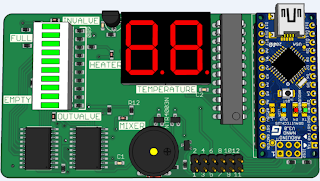
\includegraphics[height=5.5cm,width=10cm]{Figures/24.png}
	\caption{Εξομοιωτής των μηχανικών στοιχείων του σιλό \cite{Foivos}}	
\end{figure}

Το κύκλωμα διαθέτει, σύμφωνα με την [61]:
\begin{itemize}
	\item{μία μπάρα LED 10 τμημάτων για την απεικόνιση της στάθμης του υγρού ανά πάσα στιγμή μέσα στο σιλό}
	\item{δύο LED για την ένδειξη της κατάστασης των βαλβίδων εισόδου και εξόδου}
	\item{δύο LED για την ένδειξη των αισθητήρων παρουσίας υγρού}
	\item{ένα LED για την ένδειξη της κατάστασης του στοιχείου θέρμανσης και ένα LED αλλά και ένα buzzer για την ένδειξη της κατάστασης του στοιχείου μίξης}
	\item{δύο 7-segment displays για την ένδειξη της τρέχουσας θερμοκρασίας του σιλό. }
\end{itemize}

Για την επικοινωνία με τον μικροϋπολογιστή που χρησιμοποιήθηκε, χρησιμοποιήθηκαν οι διεπαφές που είχε ο εξομοιωτής του μηχανικού σιλό οι οποίες ήταν καλά ορισμένες μέσω της [61]. Από το Raspberry Pi αποστέλλονται ψηφιακά σήματα μέσω της βιβλιοθήκης Pi4J και τα γενικού σκοπού Ι/Ο που παρέχει το Raspberry Pi. 

	Είχαμε στην διάθεση μας τέσσερις εξομοιωτές του σιλό και έναν εξομοιωτή του Pipe που φαίνεται στην εικόνα 7.5. Έτσι αφού εγκαταστάθηκε το Apache Felix Framework στους μικροϋπολογιστές και έγιναν οι κατάλληλες διασυνδέσεις με τους εξομοιωτές των μηχανικών τμημάτων του σιλό το σύστημα ήταν έτοιμο για χρήση. Για την διεξαγωγή των πειραμάτων χρησιμοποιήθηκε ένα LwM2M server ο οποίος υλοποιούσε την λογική της παραγωγής και των δύο τύπων liqueur ταυτόχρονα. Ο LwM2M server είναι υλοποιημένος σε Java σαν ένα POJO και έτρεχε σε ένα Raspberry Pi 2 Model B, το οποίο απαρτίζεται από έναν τετραπύρηνο επεξεργαστή χρονισμένο στα 900MHz και από 1 Gb RAM. Η διαδικασία για την παραγωγή του liqueur τύπου Β φαίνεται στην εικόνα 7.6.
	
\begin{figure}[htbp]
	\centering
		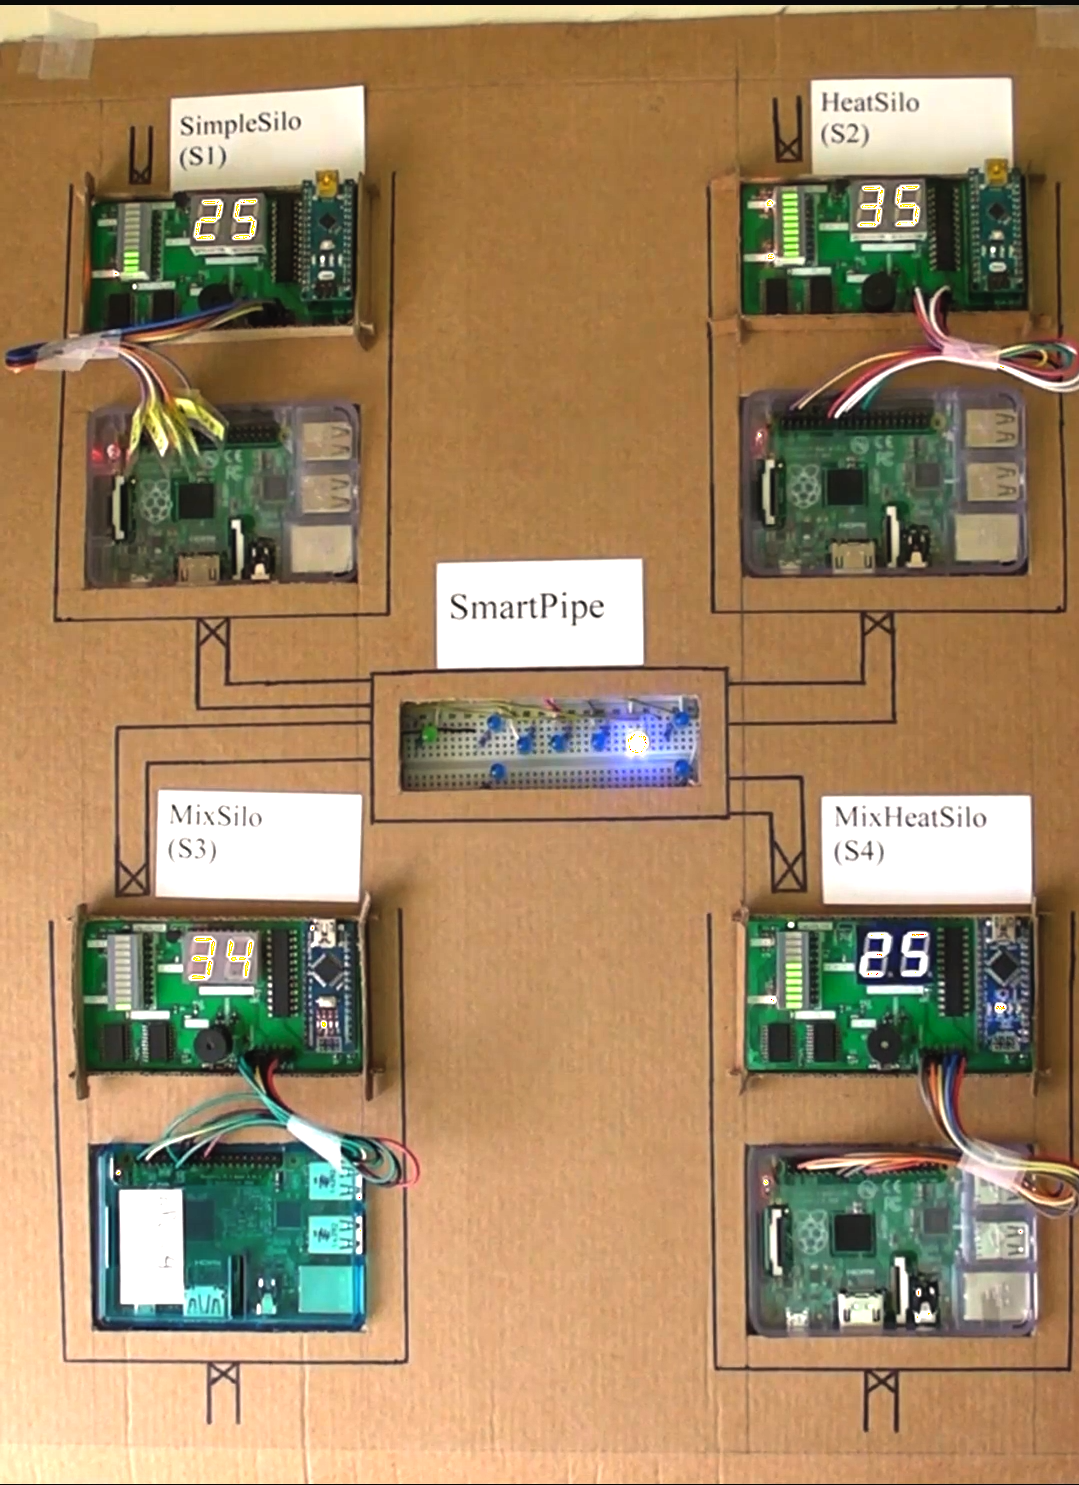
\includegraphics[height=14cm,width=10cm]{Figures/25.png}
	\caption{H πειραματική διάταξη με τα τέσσερα σιλό και τον σωλήνα}	
\end{figure}

\begin{figure}[htbp]
	\centering
		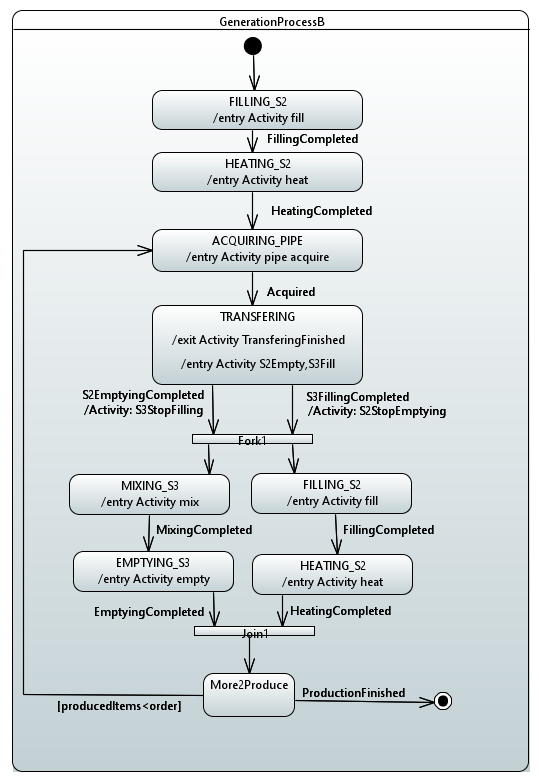
\includegraphics[height=20cm,width=14cm]{Figures/26.PNG}
	\caption{Η διαδικασία παραγωγής liqueur τύπου Β}	
\end{figure}